\subsection{SVM Kernels: But why bother duals?}

\begin{figure}[H]
\centering
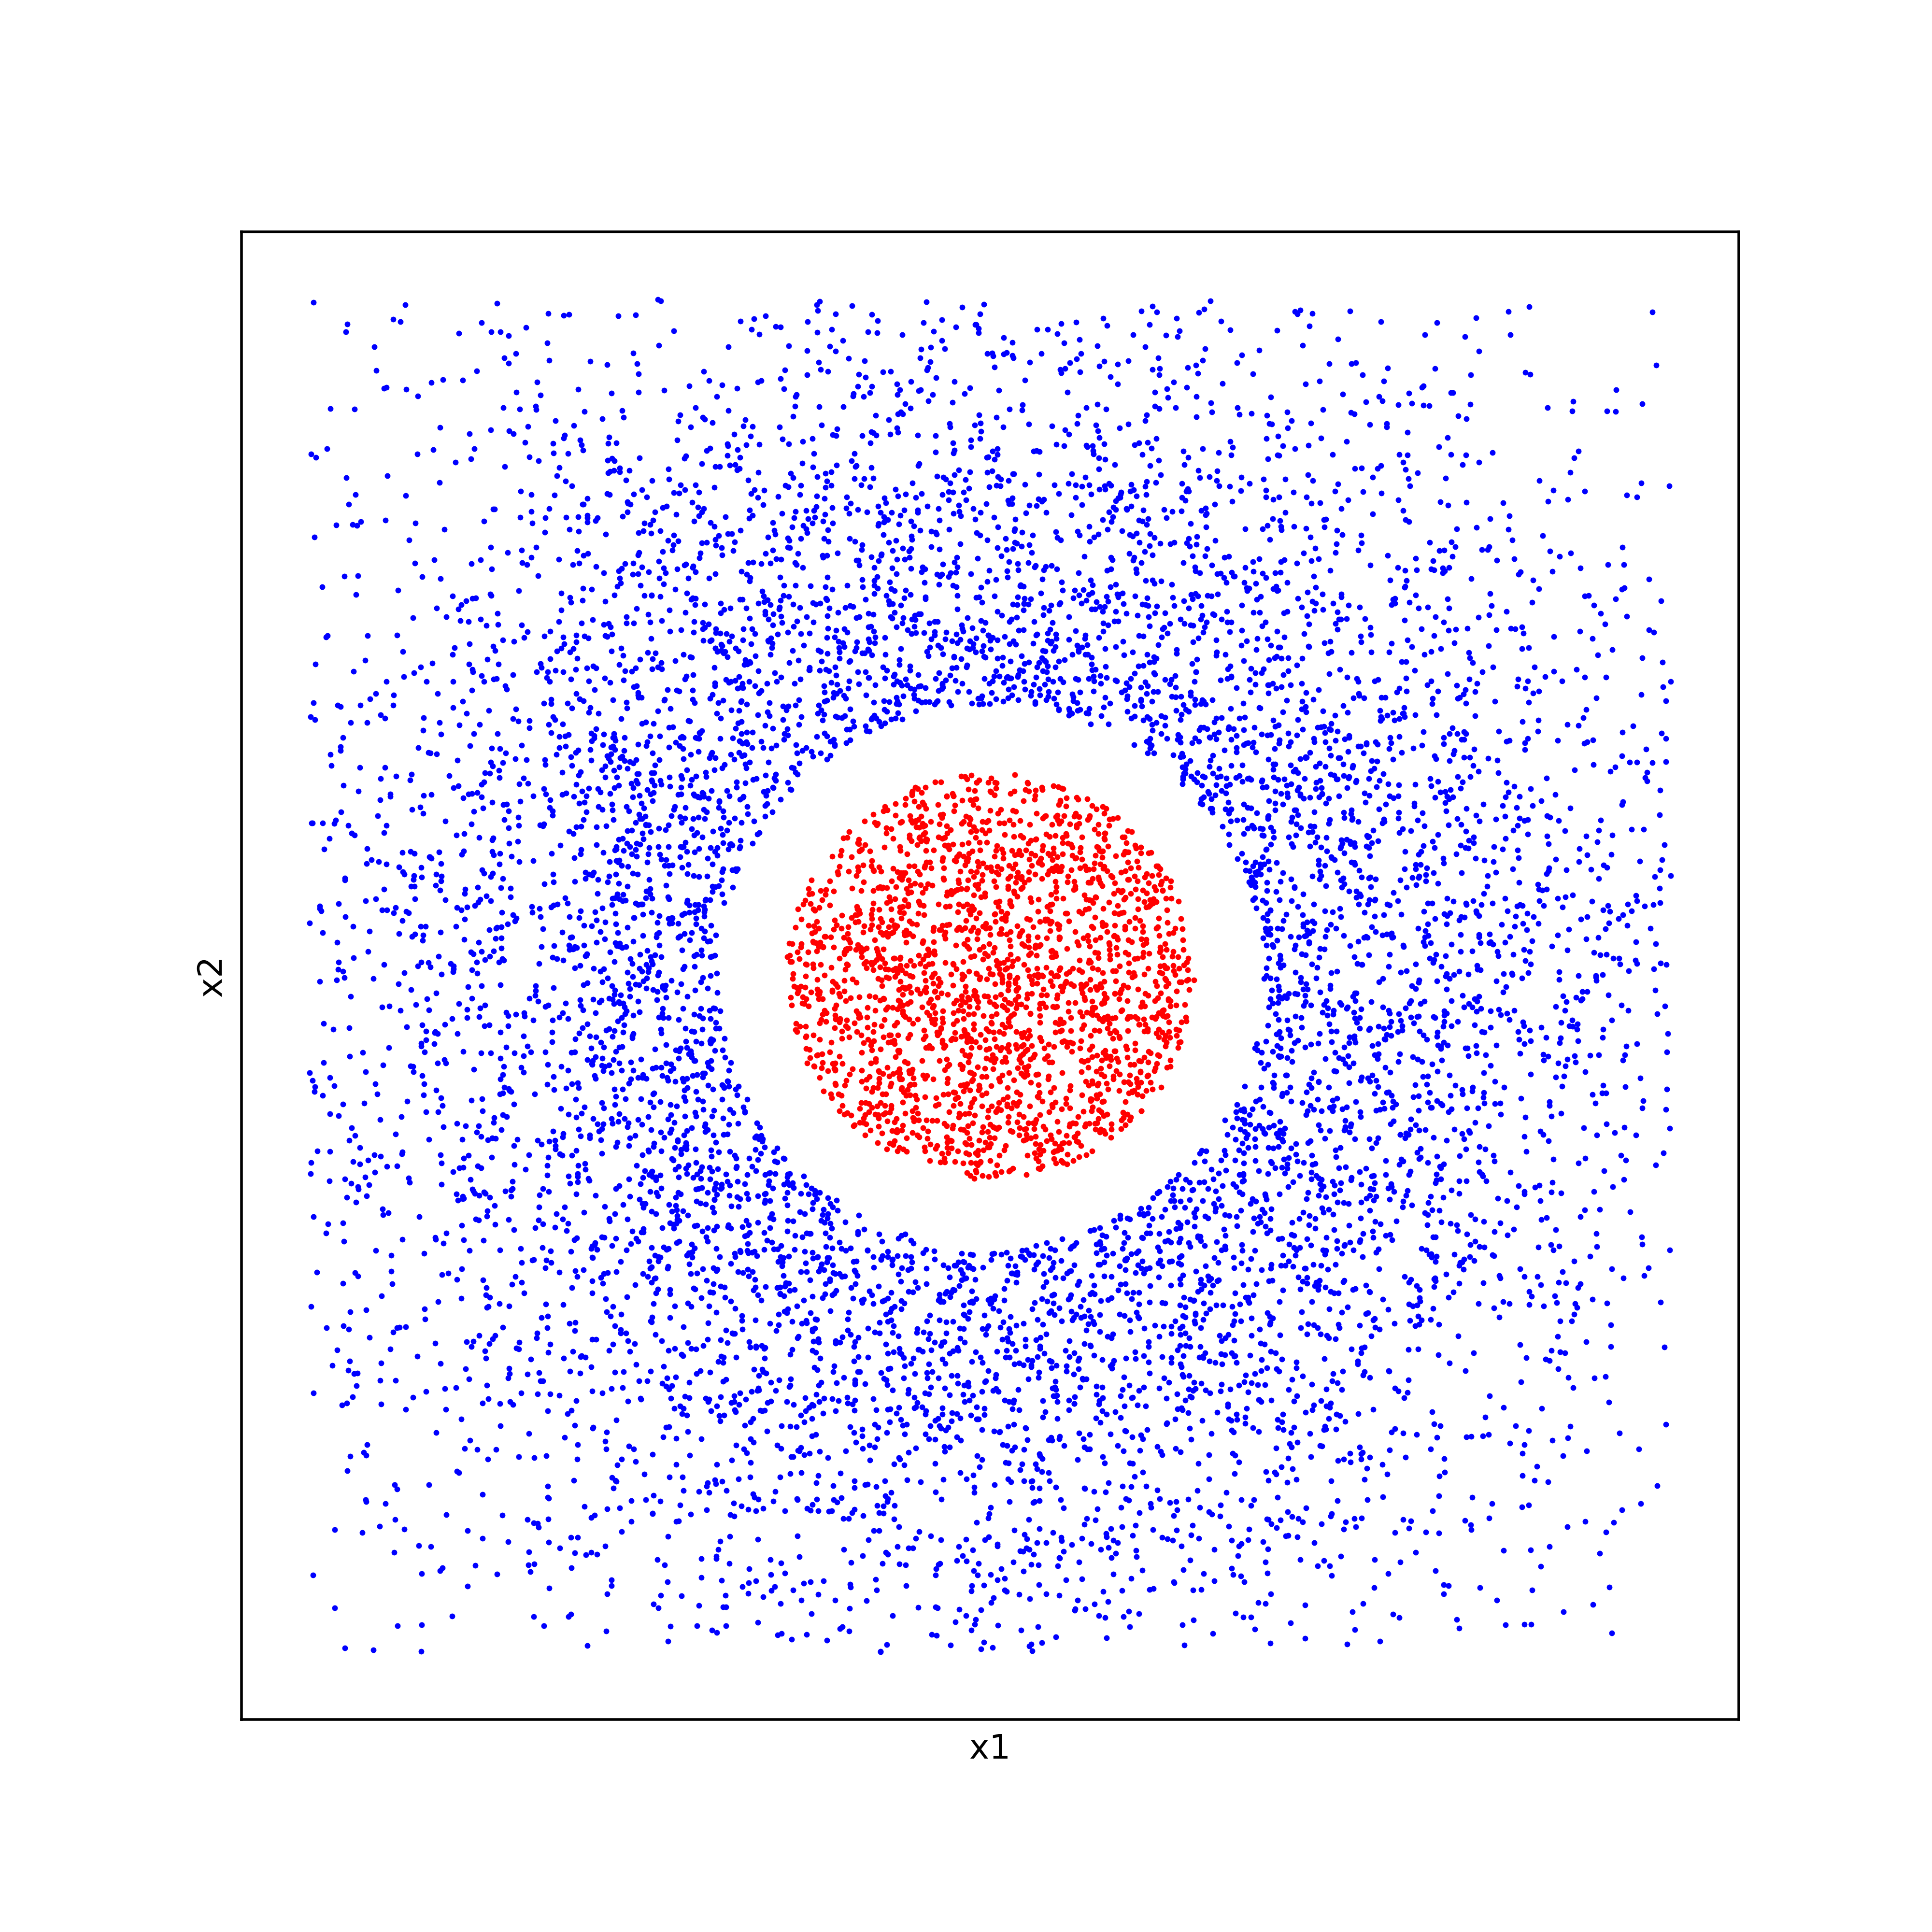
\includegraphics[width=0.5\textwidth]{images/svm.png}
\caption{Classification data for SVM}
\label{fig:svm_data}
\end{figure}
\begin{figure}[H]
    \centering
    \begin{align*}
        &\min_{\wb, b} \frac{1}{2}\norm{\wb}_2^2 \\
        &\text{s.t. } \yieg (\wb^T \xieg + b) \geq 1, \ \ i \in \{1, 2, \dots, m\}
    \end{align*}
    \caption{SVM: Primal Problem}
    \label{fig:svm_primal}
\end{figure}

\begin{figure}[H]
    \centering
    \begin{align*}
    &\max_{\alpha} \ \  W(\alpha) = \sum_{i=1}^{m} \alpha_i - \frac{1}{2} \sum_{i,j=1}^{m} y^{(i)} y^{(j)} \alpha_i \alpha_j \langle \mx^{(i)}, \mx^{(j)} \rangle\\
    &\text{s.t. } \alpha_i \geq 0,  \ \ i \in  \{1, 2, \dots, m\}\\
    &\qquad \sum_{i=1}^{m} \alpha_i y^{(i)} = 0.
    \end{align*}
    \caption{SVM: Dual Problem}
    \label{fig:svm_dual}
\end{figure}


Look at the data in \autoref{fig:svm_data}. The feature vector is expressed as $\mx = [x_1 \ \ x_2]^T$. The data is generated by sampling $\mx$ from $\mathcal{N}(\mathbf{0}, \mathbf{I})$ and filtering out points, to $|x_1| \leq 5$ and $|x_2| \leq 5$. Points within the circle with center $(0, 0)$ and radius $3$ are labeled red and those outside that of radius $4$ are labeled blue. Other points are ignored.

\begin{enumerate}[label=\alph*)]
\item Can simple SVM's (without using kernels) be used to classify the data perfectly in \autoref{fig:svm_data}.
\item Suggest a transformation $\phi: \re^2 \to \re^k$ such that when applied to the feature vectors in the data first, the data in \autoref{fig:svm_data} can be perfectly classified using SVM.

\item When the number of features is $3$, to be able to learn any quadratic decision boundary (using SVM in \autoref{fig:svm_primal}), you can use the transform 
\begin{equation*}
\phi([x_1 \ \ x_2 \ \ x_3]^T) = [x_1^2 \ \ x_2^2 \ \ x_3^2 \ \ x_1x_2 \ \ x_2x_3 \ \ x_3x_1 \ \ x_1 \ \ x_2 \ \ x_3]^T\end{equation*}
Think of a $\phi$ that can be used when $\mx \in \re^n$ and you've to be able to learn all boundaries of degree $\leq d$. What is the size of the output vector?\footnote{Hint: The number of terms in the expansion of $(x_1 + x_2 + \dots + x_n + c)^d$, $c$ is a constant.}

\item Continuing the previous part, you have a Black Box that can solve \autoref{fig:svm_primal}. What is the size of this problem, i.e. the number of coefficients in the objective and constraints. How much time does it take to compute all of them?

\item In the dual problem, notice that $\mx$ appears only in the inner product. You have been given a $\phi$ that maps $\mx \in \re^n$ to space with features, all products of ${x_1, x_2, \dots, x_n}$ of degree $\leq d$.
\begin{equation}\label{kernel}
\langle\phi(\mx), \phi(\mz)\rangle = (\mx^T\mz + c)^d
\end{equation}
$c$ is a hyperparameter that decides weight for terms of lower degrees. You have a Black Box that can solve \autoref{fig:svm_dual}. Do you realize that, given \autoref{kernel}, you do not need to worry about the exact form of $\phi$? What is the size of the problem now? How much time does it take to compute all the coefficients, without (a rough lower bound) and with the kernel trick in \autoref{kernel}?
\end{enumerate}



\subsection{Soft Margin SVM}

We have data $\mathcal{D} = \{(\xieg, \yieg)\}_{i = 1}^{m}$ where $\xieg \in \mathcal{R}^{n}$ and  $\yieg \in \{-1, 1\}$. Consider the soft SVM optimization problem

\begin{equation*}
\minbelow{\wb, b, \beps}  \ \ \loss_C(\wb, b, \beps) =  \frac{1}{1 + C} \frac{\wb^T\wb}{2} + \frac{C}{1 + C} \sum_{i = 1}^{m} \epsilon_i
\end{equation*}

Under constraints 
\begin{align*}
&y^{(i)}(\wb^T \xieg + b) \geq 1 - \epsilon_i \ \ i \in \{1, 2, \dots, m\}\\
&\epsilon_i \geq 0  \ \ i \in \{1, 2, \dots, m\}
\end{align*}

Denote \(\beps = [\epsilon_1 \ \  \epsilon_2 \ \  \dots \ \  \epsilon_m]^T\). \(C \geq 0\) is a hyperparameter.
In each of the below cases, give the optimum value of the objectives and construct the exact values of $\wb, b, \beps$ that lead to that objective.
\begin{enumerate}[label=\alph*)]
\item $\loss_0(\wb, b, \beps)$
\item $\loss_{\infty}(\wb, b, \beps)$ when $\mathcal{D}$ is linearly separable.
\item Comment on the value of objective $\loss_{\infty}(\wb, b, \beps)$ when $\mathcal{D}$ is \textbf{not} linearly separable.
\end{enumerate}



